\documentclass[12pt]{article}

\usepackage{mathptmx}

\usepackage[colorlinks=true,urlcolor=blue]{hyperref}
\urlstyle{same}


\usepackage{graphicx}
\graphicspath{{./figures/}}

\usepackage[outdir=./figures/]{epstopdf}

\usepackage{float}

\usepackage[font=footnotesize]{caption}

\usepackage{wrapfig}

%\usepackage[a4paper]{geometry}

\usepackage{microtype}

\usepackage{booktabs}



\author{Gabriel Siqueira Kakizaki}
\date{\today}
\title{\textbf{Relationship Between Venue Categories and Income in Districts of
the City of São Paulo, Brazil}}

\begin{document}
\maketitle



\section{Introduction}

\subsection{Background}

São Paulo, according to the Globalization and World Cities (GaWC) Research
Network, is an alpha global city, along with Los Angeles and Amsterdam. It is
in the ranking of the wealthiest and the most populous cities of the world,
known for its cultural, social and ethnic diversity. Often holding
international events, it is sought-after because of its opportunities for
business.

\subsection{Problem}

Opening a new business in such place can be challenging by a number of reasons.
Choosing a location in itself has a number of things to consider, and the
income of people living in the surrounding area might be one of them. The aim
of this project is to discover, if any, the relation between the type of venue
and the income of people living in the districts of the city of São Paulo.

\subsection{Stakeholder interest}

The main audience of this project are entrepreneurs choosing where to open a
business in São Paulo. The results could also be useful for people just wanting
to move to the city, real estate agents, and investors because this information
might give an edge on decision-making.



\section{Data}

\subsection{Data sources}

Income and geographic data came from IBGE (Brazilian Institute of Geography and
Statistics), and can be accessed
\href{https://www.ibge.gov.br/en/home-eng.html}{here}. More specifically, the
income data comes from the 2010 Population Census (to know more about click
\href{https://www.ibge.gov.br/en/statistics/social/income-expenditure-and-consumption/18391-2010-population-census.html?=&t=o-que-e}{here}),
and geographic data comes from
\href{https://www.ibge.gov.br/geociencias/organizacao-do-territorio/malhas-territoriais/26565-malhas-de-setores-censitarios-divisoes-intramunicipais.html?=&t=o-que-e}{here}
(portuguese) in form of shapefiles for geographic information system (GIS)
software.  Venue data was gathered using the
\href{https://developer.foursquare.com/places}{Foursquare Places API} with a
free account created for this project.

\subsection{Data description}

\subsubsection{Geographic data}

The shapefiles came with information about the district boundaries, along with
its name, code and id. This data covered the whole state of São Paulo, not just
the city. A sample of it is shown in \autoref{fig:geopandas}.

\begin{figure}[h]
        \centering
        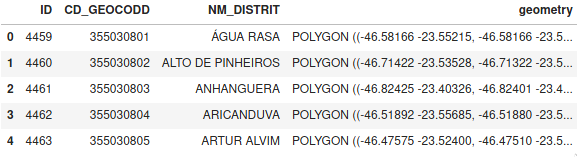
\includegraphics[width=0.8\textwidth]{geopandas.png}
        \caption{Geopandas dataframe\label{fig:geopandas}}
\end{figure}

\subsubsection{Census data}

The census table contained various attributes, and the statistics columns were
labeled with ``VXXX'', where XXX is a three-digit number. The relationship
between labels and their meaning can be found on the 2010 census documentation.

As we were interested only on the income, only the column ``V009'' was used,
which translating its name to english means: ``Value of the average nominal
monthly income of persons aged 10 and over (with and without income)''. There
weren't any missing values for this column.

Originally, each row is associated with a unit called ``census sector''
(portuguese: setor censitário), which is normally a lot smaller than the actual
district, composed only of one or a few city blocks.

A part of this table can be seen in \autoref{fig:census_table}.

\begin{figure}[h]
        \centering
        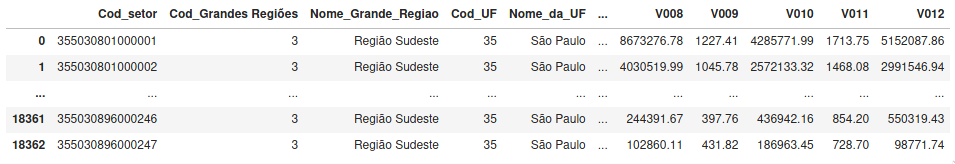
\includegraphics[width=\linewidth]{census_table.png}
        \caption{Pandas dataframe containing the census data.\label{fig:census_table}}
\end{figure}

\subsubsection{Venues}

Foursquare API was used to collect the name, category, latitude and longitude
values for a total of 8036 venues in a 2 km radius around the centroid of each
of the 96 districts. The results returned from the API in JSON format were
merged into a dataframe containing the district name, and coordinates as shown
in \autoref{fig:venues_table}.

\begin{figure}[h]
        \centering
        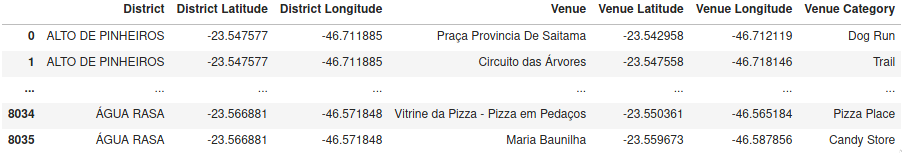
\includegraphics[width=\linewidth]{venues_table.png}
        \caption{Pandas dataframe containing the venue information.\label{fig:venues_table}}
\end{figure}



\section{Methods}

All data processing, analysis and modeling was done using Python and various
libraries. This work can be seen in a Jupyter notebook at my github page
(\href{https://github.com/kakig}{github.com/kakig}) on the repository
\verb!Coursera_Capstone!.

\vfill

\subsection{Exploratory data analysis (EDA)}

\begin{wrapfigure}{L}{0.5\textwidth}
        \centering
        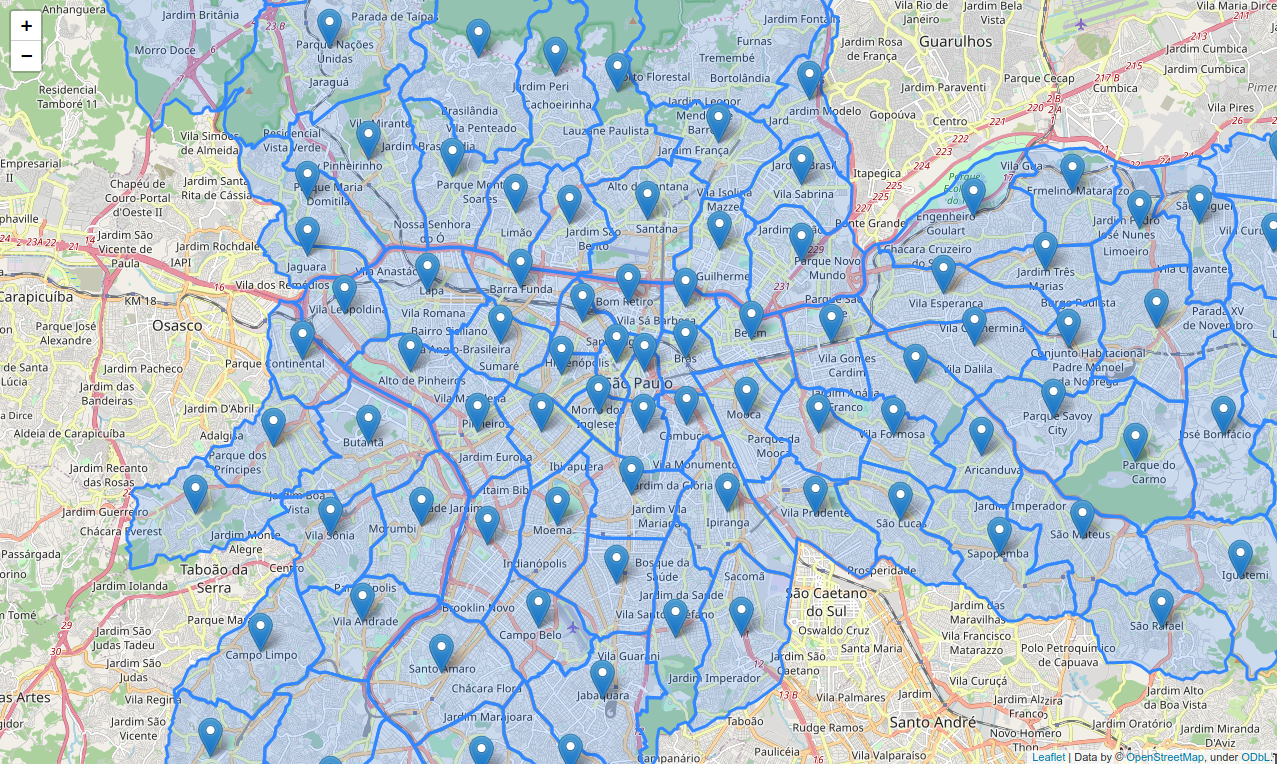
\includegraphics[width=\linewidth]{map_centroids.png}
        \caption{Map of São Paulo showing districts with markers on its
        centroids.\label{fig:map_centroids}}
\end{wrapfigure}

As shapefiles came with information for the whole state, only data about the
city was selected. Then, centroids were calculated for each district using its
geometry information, for use with the Foursquare API.\spacefactor\sfcode`.{}
Some conversion between different coordinate reference systems (CRS) was needed
for this calculation and for plotting maps, which also required generating a
GeoJSON object. To verify that the area and placement of the districs and the
calculated centroids were correct, a map was created for visualization, as
shown in \autoref{fig:map_centroids}.


Proceeding to census data, to get the average income per district instead of
per census sectors, data was grouped by district name and the mean was taken.
The mean income for the districts was R\$1576.82, and the minimum and maximum
as R\$396.48 and R\$5402.81 respectively. There are few outliers, but they are
not very large and should not disturb our analysis. The distribution of the
values can be seen in \autoref{fig:plot_income}.

\begin{figure}[htb]
        \centering
        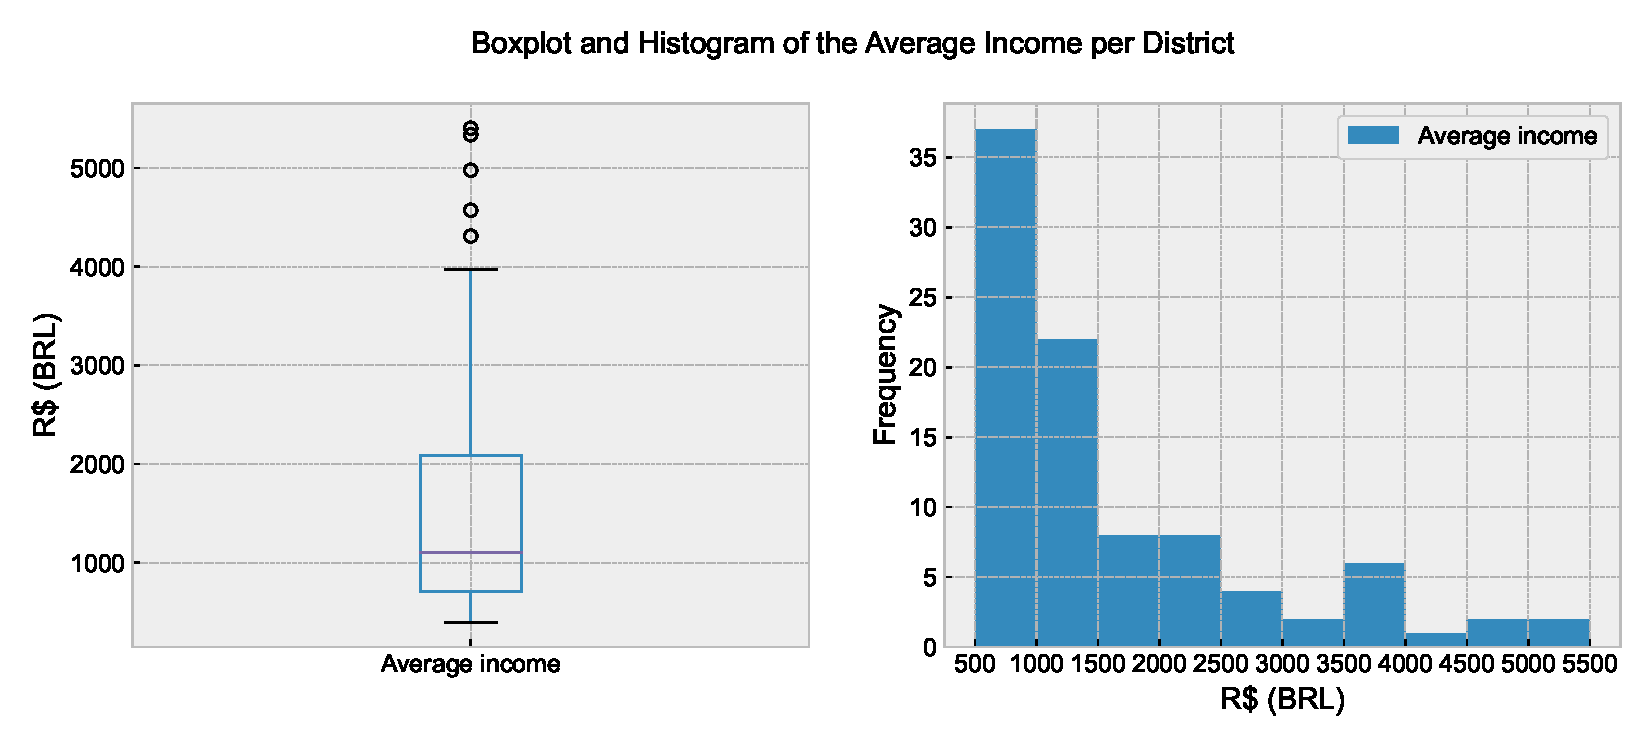
\includegraphics[width=\linewidth]{plot_income.eps}
        \caption{Boxplot (left) and histogram (right) of income. Values in
        Brazilian Real.\label{fig:plot_income}}
\end{figure}

\begin{wrapfigure}{R}{0.5\textwidth}
        \centering
        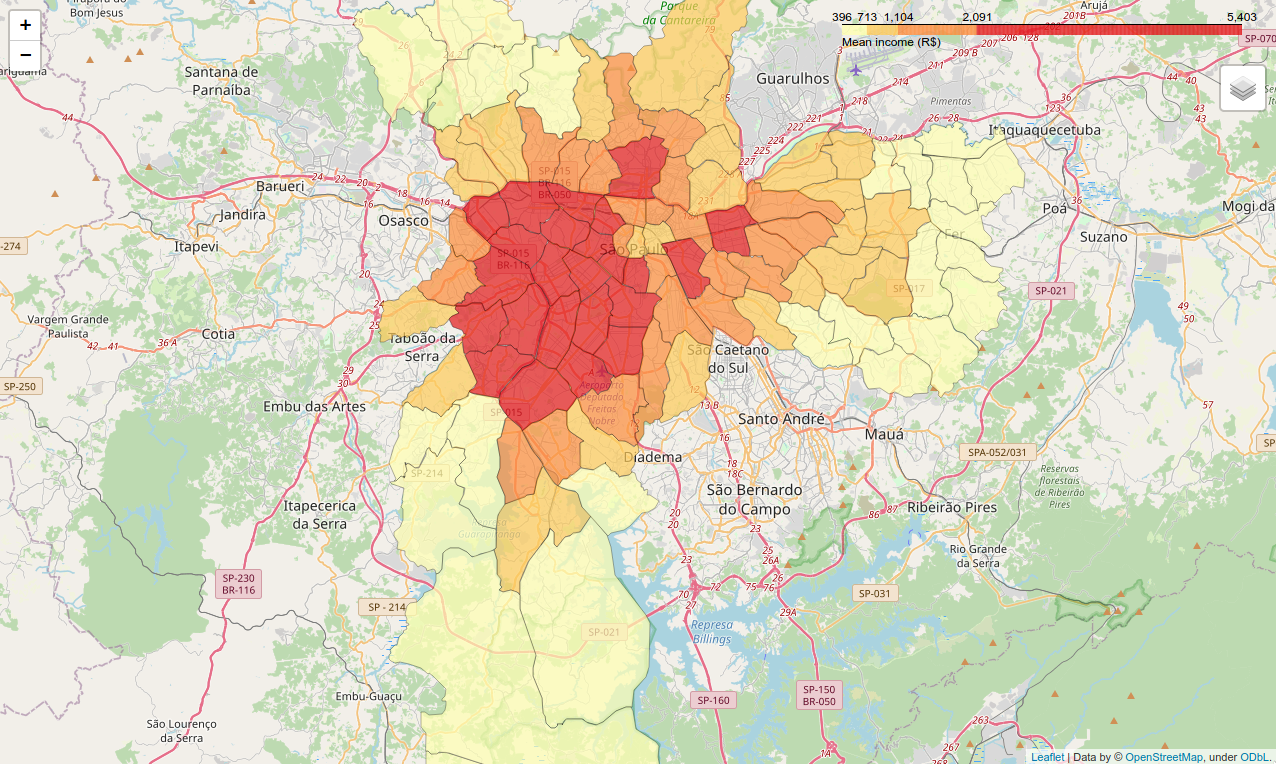
\includegraphics[width=\linewidth]{map_income.png}
        \caption{Average income per district of São Paulo. Red means higher
        income.\label{fig:map_income}}
\end{wrapfigure}

Joining the income with geographical data, it is possible to visualize where
the income is higher or lower. In \autoref{fig:map_income} we could observe that
higher income is more concentrated to the center of the city, and lowers as we
go far from the center. If the income has no impact on the type of venues, then
we should see the same, or at least close frequencies of venues across the
districts. If it does make a difference, and that is our hypothesis, we should
see different ratios of venues across different income ranges.

Switching focus to working with venue information, due to the difference in
number of venues between districts, first, one-hot encoding was used to
transform the table, keeping only the category value for each venue. There were
363 unique venue categories that became the columns for the table. Data in this
format was used to visualize the most common venues in the whole city. Then, the
values were grouped by district with and the mean was taken, so we ended up with
the frequency of venue categories in percentage for each district. This may
allow for a better and more fair comparison during modeling.

\subsection{Modeling}

Machine learning models were built using the
\href{https://scikit-learn.org/stable/index.html}{scikit-learn} library. Both
unsupervised (K-Means) and supervised (Lasso, Random Forest) learning approaches
were used in a complementary manner.

\begin{wrapfigure}{l}{0.5\linewidth} \centering
        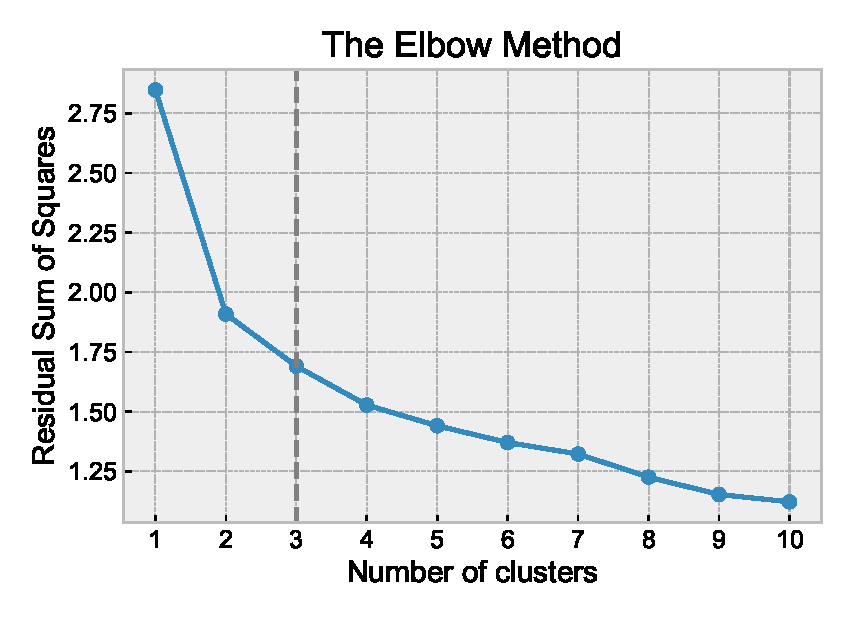
\includegraphics[width=\linewidth]{plot_elbow.eps}
        \caption{Elbow method for choosing the number of clusters in
        K-Means\label{fig:plot_elbow}}
\end{wrapfigure}

K-Means algorithm was used to segment \emph{n} data points (districts) into
\emph{K} segments, or clusters, with similar characteristics (venue frequency).
Note that income data \textbf{was not} used to train this algorithm. As it
cannot automatically determine the number of clusters in the data, the elbow
method was used for choosing the optimal \emph{K}, which was three in this
case.

The target of prediciton for regression was the mean income for each district.
Due to our sample size, models were evaluated using \emph{k-fold}
cross-validation (\(k=5\)) to estimate the coefficient of determination (R²),
mean absolute error (MAE) and root mean squared error (RMSE).

Lasso was used instead of ordinary least squares regression due to the large
number of features (363 venue categories), as it tends to have fewer non-zero
coefficients, thus being simpler.

Random forest was also used because the data might have a non-linear
relationship, so a decision tree model can better fit the data and it still can
be used to explain feature importances.



\section{Results}

\subsection{Clustering}

K-Means segmented the districts mainly into 2 clusters, and the third cluster
contained only one district, the most southern one which contains an
environmental preservation area, and because of that it was excluded from
further analysis.

\begin{figure}[h]
        \centering
        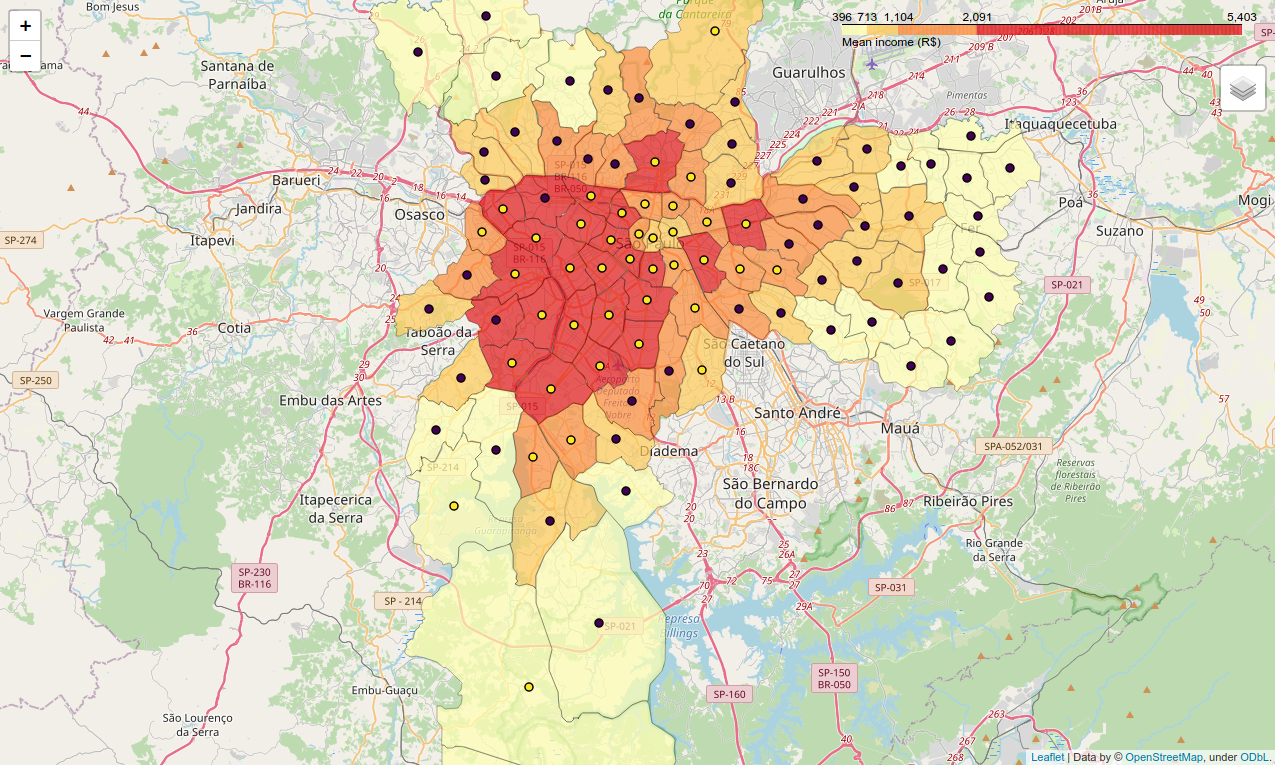
\includegraphics[width=\linewidth]{map_cluster_labels.png}
        \caption{Choropleth map of income per district. Dark purple circles
        indicate the district is part of the first cluster, and yellow circles,
        the second.\label{fig:map_cluster_labels}}
\end{figure}

\newpage

The first cluster had 55 districts with a mean income of R\$924.24 and the
second had 40 districts, and a mean income of R\$2503.62, more than double than
the first one. The first cluster also had mostly bakeries and pizza places as
most common venues, while the second had a more diverse selection of most
common venues. As can be seen in \autoref{fig:map_cluster_labels}, districts
from the second cluster are usually located more to the center.

%\autoref{tab:clusters} shows the number of districts and the income for the
%first two clusters. The first cluster had 55 districts with a mean income of
%R\$924.24 and the second had 40 districts, and a mean income of R\$2503.62,
%more than double than the first one. The first cluster also had mostly bakeries
%and pizza places as most common venues, while the second had a more diverse
%selection of most common venues.

%\begin{table}[h]
%        \centering
%        \begin{tabular}[c]{ c c c }
%                \toprule
%                Cluster & Districts & Mean Income (R\$) \\
%                \midrule
%                1 & 55 & 924.24 \\
%                2 & 40 & 2503.62 \\
%                \bottomrule
%        \end{tabular}
%        \caption{Number of districts and mean income from clusters\label{tab:clusters}}
%\end{table}

\subsection{Regression}

\begin{table}[h]
        \centering
        \begin{tabular}[c]{ c c c c }
                \toprule
                Model & R² (mean, std) & MAE & RMSE \\
                \midrule
                Lasso & 0.53 (0.19) & 615 & 810 \\
                Random Forest & 0.58 (0.15) & 566 & 752 \\                \bottomrule
        \end{tabular}
        \caption{Coefficient of determination, mean absolute error and root
        mean squared error for lasso and random forest
        models.\label{tab:models}}
\end{table}

\autoref{tab:models} shows the performance of the two regression models. Random
forests performed better lasso in all metrics, thus it was used to explain
which venue categories are correlated with high and low income districts using
SHAP values as shown in \autoref{fig:plot_shap_rf}. We can see that higher
bakery frequency tends to lower the value of the predicted income, confirming
what was shown with clustering. In general, restaurants of different (foreign)
cuisines tend to increase the value of the output of the model, indicating that
they are located in higher income areas.

It is also interesting to see that spa, vegetarian/vegan restaurant and art
museum categories impact positively the model output, reinforcing the common
sense conception that these places are frequented by people with higher
economic status.

\begin{figure}[h]
        \centering
        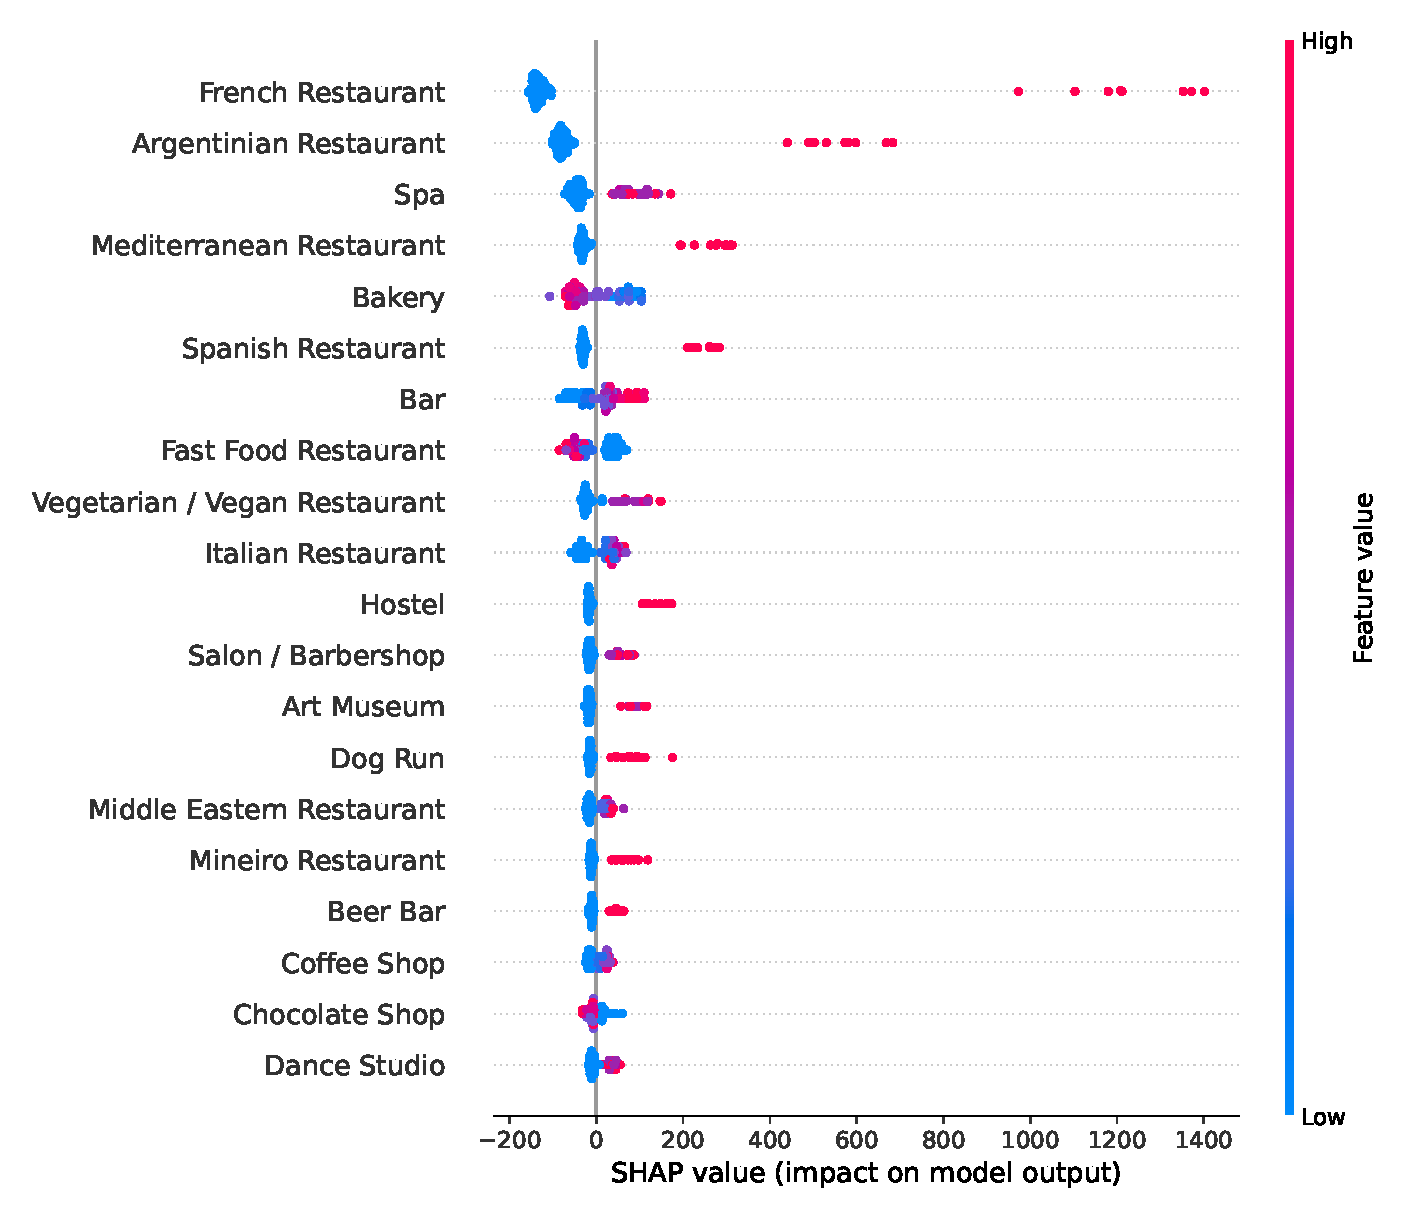
\includegraphics[width=\linewidth]{plot_rf_shap.eps}
        \caption{SHAP values for the top 20 features sorted by average impact
        on model output.\label{fig:plot_shap_rf}}
\end{figure}



\section{Discussion}

\subsection{Recommendations}

For further research, the relationship between venue types and other kinds of
data could be explored, such as with crime rates, renting prices, etc. This may
lead to other insights about venue localization and where it might be best to
open a new place. Also, using a smaller terrain unit than a district could be
useful for pinpointing more exact locations suited for opening a new business.

While working with geographical data, caution should be used to verify that the
information about all places is correct. I had problems with districts, and
previously with neighborhoods that had the exact same name in this and other
cities. Also the names can contain abbreviations and sometimes do not match
where they should.

\subsection{Limitations}

The census data was gathered in 2010, and venue data is from 2020. This may
impact the models accuracy and the explanations of which venue types are
correlated with higher or lower income areas.

Venue data was gathered in a 2 km radius from the districts centroid, because
the Foursquare API is limited to a circular search around latitude and
longitude coordinates. This 2 km radius is good for most of the districts, but
this selection isn't perfect. The venue data for smaller districts agglomerated
in the center may have included venues in other adjascent districts, and
districts at the edge of the city might have venues from other cities, due to
conurbation. While I could have restricted venues to be inside of the district,
this would result in less data for the machine learning algorithms, and in
practice, these kinds of political divisions aren't really obstacles for people
going to the venues.

\section{Conclusion}

In this study I analyzed the relationship between the venue categories and the
income for districts of city of São Paulo, and identified that few venue
categories are correlated to the income, especially restaurants from foreign
cuisine. It is also worth noting that bakeries and fast food restaurants appear
more in lower income areas. This information could be useful to help
entrepreneurs deciding the location of a new business, to know better their
public based on the income.

\end{document}
